\documentclass[12pt,oneside]{article}
\usepackage{geometry}
	\geometry{a4paper,inner=2cm, outer=3cm, top=3cm, bottom=3cm}

\usepackage[bitstream-charter]{mathdesign}
\usepackage[T1]{fontenc}

\usepackage[usenames, dvipsnames]{color}
\usepackage{titlesec}
    \titleformat{\section}
        {\color{RoyalBlue}\normalfont\Large\bfseries}
        {\color{RoyalBlue}\thesection}{1em}{}

\usepackage{pdfpages}
\usepackage{hyperref}
\makeatletter
\renewcommand*\l@section{\@dottedtocline{1}{1.5em}{2.3em}} % dots in the table of contents
\makeatother

\newcommand{\oporcom}[1]{\texttt{\color{RoyalBlue}#1}} % simplified the highlighting of options and commands in text
\newcommand{\comoptions}[1]{\texttt{\color{Gray}#1}} % simplified the highlighting of options and commands in text

\setcounter{secnumdepth}{0}

\begin{document}
    
\title{\textbf{The \texttt{uowthesistitlepage} Package\\
Redefinition of \texttt{\textbackslash{}maketitle} to Create a Title Page for a Thesis at the University of Wollongong}}
\author{Thomas M. Griffiths}
\date{Released \today, Version 1.1}

\maketitle

\tableofcontents

\section{About}
This package redefines the \oporcom{\textbackslash{}maketitle} command for LaTeX documents and generates a title page compliant with the UOW branding guidelines. Also in this package is a new command \oporcom{\textbackslash{}declaration} which typeset a declaration page required in the frontmatter of each PhD thesis. Use this package with the book class to typeset your thesis. The package has a number of options that change the wording of the title page according to: whether your thesis is part of, or the entire component of assessable work for your degree; the number of supervisors you have, if any. This package \emph{is not} a complete thesis template or document class, it only typesets the title page. The default options when the package is loaded are: \oporcom{honours} and \oporcom{onesupervisor}

\section{Legal}
This work is copyright (CC BY-NC-SA 3.0 AU) 2013 by T. M. Griffiths under the creative commons licence (attribution, non-comercial, share alike). More information can be found here: \url{http://creativecommons.org/licenses/by-nc-sa/3.0/au/}. 

This work may be distributed and/or modified under the conditions of the LaTeX Project Public License version 1.3c which can be found at: \url{http://www.latex-project.org/lppl/lppl-1-3c.txt}.

The crest of the University of Wollongong is copyright and the property of the University of Wollongong. As the core identifier of the university its use is governed by the university's brand and visual identity guidelines which can be found at: \url{http://www.uow.edu.au/about/brand/uowlogo/index.html}

\section{Usage}
\subsection*{\oporcom{\textbackslash{}maketitle}}
If you are familiar with LaTeX using this package is very simple, place the \texttt{uowthesistitlepage} package in your document's preamble:
\begin{verbatim}
\usepackage[]{uowthesistitlepage} 
\end{verbatim}
The standard parts of the \oporcom{\textbackslash{}maketitle} command still apply. The title, author and date fields are filled in as normal, the package uses them in the title page.
\begin{verbatim}
\begin{document}
\title{A Pretty Swish Title} 
\author{Average J. Blow}
\date{Month Year}
\end{verbatim}
The new fields from the uowthesistitlepage package are\oporcom{\textbackslash{}degree}, \oporcom{\textbackslash{}school} and \oporcom{\textbackslash{}supervisor}. They're fairly self-explanatory and you use them just as you would the standard macros for the regular \oporcom{\textbackslash{}maketitle} command.  
\begin{verbatim}
\degree{That Degree You've Been Studying} 
\school{Your School} 
\supervisor[x]{Supervisor 1, Supervisor 2 \& Supervisor 3 etc.}
\end{verbatim}
You need to ensure a copy of the logo named \texttt{uow\textunderscore{}logo} is in the working directory where you're compiling your thesis, if you downloaded this style from the UOW website there will be one in the zipped package. When you want to typeset the title page simply use \oporcom{\textbackslash{}maketitle} after all the defined fields as you usually would.

\subsection*{\oporcom{\textbackslash{}declaration}}
Using the \oporcom{\textbackslash{}declaration} command is simple just place it in your document where you want it typeset. It uses the same macros (\oporcom{\textbackslash{}author}, \oporcom{\textbackslash{}degree} and \oporcom{\textbackslash{}school}) that we defined for the redefinition of \oporcom{\textbackslash{}maketitle}. 


\section{Package Options and Macros}
\subsection*{Macros}
\begin{description}
    \item[\oporcom{\textbackslash{}author}\comoptions{\{Your Name\}}]
    The author of the work, in this case you. For the your thesis you should use your full name and any previous degrees, for example: Average Joe Blogs BSc Hon.
    
    \item[\oporcom{\textbackslash{}date}\comoptions{\{Month Year\}}]
    The date of your submission, usually `Month Year'. Alternatively, you can use the \oporcom{\textbackslash{}today} macro, and it will print the date in the format month dd, yyyy.
    
    \item[\oporcom{\textbackslash{}declaration}] This typesets the declaration that is required in the frontmatter of a PhD thesis. It's used in the exact same way as \oporcom{\textbackslash{}maketitle}, place it in the document where you want it typeset, and it will typeset the following:
\begin{quote}
    \noindent {\large \textbf{Declaration}}\\

    \noindent I, \textless{}Student's Full Name\textgreater, declare that this thesis, submitted in fulfilment of the requirements for the award of \textless{}Your Degree\textgreater, of the School of \textless{}Your School\textgreater, University of Wollongong, is wholly my own work unless otherwise referenced or acknowledged. The document has not been submitted for qualifications at any other academic institution.\\
    \vspace{16mm}\\
    \noindent\rule{0.4\textwidth}{1pt}\\
    \vspace{8mm}\\
    \textbf{\textless{}Student's Full Name\textgreater}, \today\\
\end{quote}
    
    \item[\oporcom{\textbackslash{}degree}\comoptions{\{Your Degree\}}]
    The degree for which you are submitting this work. Write the degree out in full; Doctor of Philosophy, Master of Science, Bachelor of Arts Honours etc.
    
    \item[\oporcom{\textbackslash{}graphic}]
    This macro is used internally to load the UOW Graphic. It has no immediate use in the body of your document and can be ignored unless you feel like cracking open the style file and tinkering. For the graphic to load properly in the title page there must be an image file in the working directory named \texttt{uow\textunderscore{}logo}. It can be used in the body of the document to load an alternative graphic if that is desired, be warned that determining the size in this case is up to you.
    The usage is a bit odd note the nested \oporcom{\textbackslash{}includegraphics} command:
    
    \oporcom{\textbackslash{}graphic}\comoptions{\{\textbackslash{}includegraphics\{yourgraphic\}\}}
    
    \item[\oporcom{\textbackslash{}requirement}]
    Similar to the \oporcom{\textbackslash{}graphic} macro, this macro is for internal use. It is manipulated by the degree options (\oporcom{phd}, \oporcom{honours} etc.) in the preamble, and determines what is printed in the requirement section of the title page. The default is the \oporcom{honours} option.
    
    \item[\oporcom{\textbackslash{}school}\comoptions{\{Your School\}}]
    The school within the university with which you are associated. If you are not associated with a school you can use the \oporcom{noschool} option in the preamble to disable the school under the UOW logo. The \oporcom{\textbackslash{}school} command will still work with the \oporcom{noschool} option, so you can specify another affiliation, for example The Australian Institute for Innovative Materials (AIIM).
    
    \item[\oporcom{\textbackslash{}supervisor}\comoptions{[number of supervisors (integer)]\{Your Supervisors\}}]
    Prints your supervisor(s) to the title page. List all your supervisors and their titles in the one set of enclosing braces (\texttt{\{ \}}), separated by commas with an ampersand (\&) before the final supervisor if you have multiple supervisors. Use the optional argument `\texttt{[x]}' to specify how many supervisors you have. The default number of supervisors is one.
    
    \item[\oporcom{\textbackslash{}title}\comoptions{\{Your Thesis Title\}}]
    Self explanatory, it's the title of your thesis
\end{description}

\subsection*{Options}
\begin{description}
    \item[\oporcom{honours}]
    One of the degree options and the default. This option modifies the wording of the thesis requirement so that it is reflective of an honours degree: `This thesis is presented as part of the requirement for the'.
    
    \item[\oporcom{honors}]
    Identical to \oporcom{honours}, just the alternative u-less spelling. See above.
    
    \item[\oporcom{phd}]
    One of the degree options. This option modifies the wording of the thesis requirement so that it is reflective of a Doctoral degree: `This thesis is presented as required for the'.
    
    \item[\oporcom{mastersbyresearch}]
    One of the degree options, the same as \oporcom{phd}. This option modifies the wording of the thesis requirement so that it is reflective of a Masters by Research: `This thesis is presented as required for the'.
    
    \item[\oporcom{mastersbycoursework}]
    One of the degree options, the same as \oporcom{mastersbyresearch} except that the thesis is only a partial requirement for the award of the degree. This option modifies the wording of the thesis requirement so that it is reflective of a Masters by Coursework: `This thesis is presented as part of the requirement for the'.
    
    \item[\oporcom{multiplesupervisors}]
    Makes the supervisor field plural, printing `Supervisors'. Still implemented but unnecessary, use the optional argument to the \oporcom{\textbackslash{}supervisor} command.
    
    \item[\oporcom{noschool}]
    Removes the text underneath the UOW stating your school affiliation. While it removes the `School of' text it doesn't deactivate the \oporcom{\textbackslash{}school} command completely it prints an empty space instead. The \oporcom{\textbackslash{}school} command will still works with the \oporcom{noschool} option, so that you can specify another affiliation.
    
    \item[\oporcom{nosupervisor}]
    Removes the supervisor field from the title page completely. Incorporated mainly to match the Word template, which, oddly is missing a supervisor field. Still implemented but unnecessary, use the optional argument to the \oporcom{\textbackslash{}supervisor} command
    
    \item[\oporcom{onesupervisor}]
    Makes the supervisor field singular, printing `Supervisor' This option is the default. Still implemented but unnecessary, use the optional argument to the \oporcom{\textbackslash{}supervisor} command
\end{description}

\section{Change Log}
If you spot any errors or bugs, or alternately you have any requests for an addition let me know.
\subsubsection*{Version 1.1, 2013-07-01, tmgriffiths}
\begin{itemize}
    \item Rewrote the \oporcom{\textbackslash{}supervisor} command to have an optional argument giving the number of supervisors. I used the \texttt{etoolbox} package and its \texttt{\textbackslash{}ifnumcom} macros to do so. The old options \oporcom{nosupervisor}, \oporcom{onesupervisor} and \oporcom{multiplesupervisors} still exist but mainly for legacy reasons. It is not necessary to specify them in the preamble anymore. The only thing of note is that \oporcom{nosupervisor} is achieved by either \oporcom{nosupervisor} in the preamble or \oporcom{\textbackslash{}supervisor}\texttt{[0]\{\}} in the document Simply leaving out supervisor will not remove the field.
    \item Rewrote the way each degree type specified partial or complete requirement in the \oporcom{\textbackslash{}@requirement} macro. I'm now using \texttt{\textbackslash{}if} statements to set the field.
    \item Implemented the \oporcom{\textbackslash{}declaration} command (see examples). It typesets declaration page that PhD students are required to have in the frontmatter of their thesis.
\end{itemize}

\subsubsection*{Version 1.0, 2013-23-06, tmgriffiths}
\begin{enumerate}
    \item Implimented \oporcom{phd}, \oporcom{mastersbyresearch}, the various \oporcom{supervisor} based, and \oporcom{noschool} options.
    \item Annotated code in sty file.
    \item Wrote documentation.
\end{enumerate}

\section{Example Title Pages}
In order on the following pages they are:
\begin{enumerate}
    \item \oporcom{onesupervisor,honours} \emph{default}
    \item \oporcom{multiplesupervisors,phd}
    \item \oporcom{nosupervisor,phd}
    \item \oporcom{noschool,honours}
    \item Microsoft Word 2010 template for comparison.
    \item \oporcom{\textbackslash{}declaration} declaration page (mainly for PhD theses).
\end{enumerate}
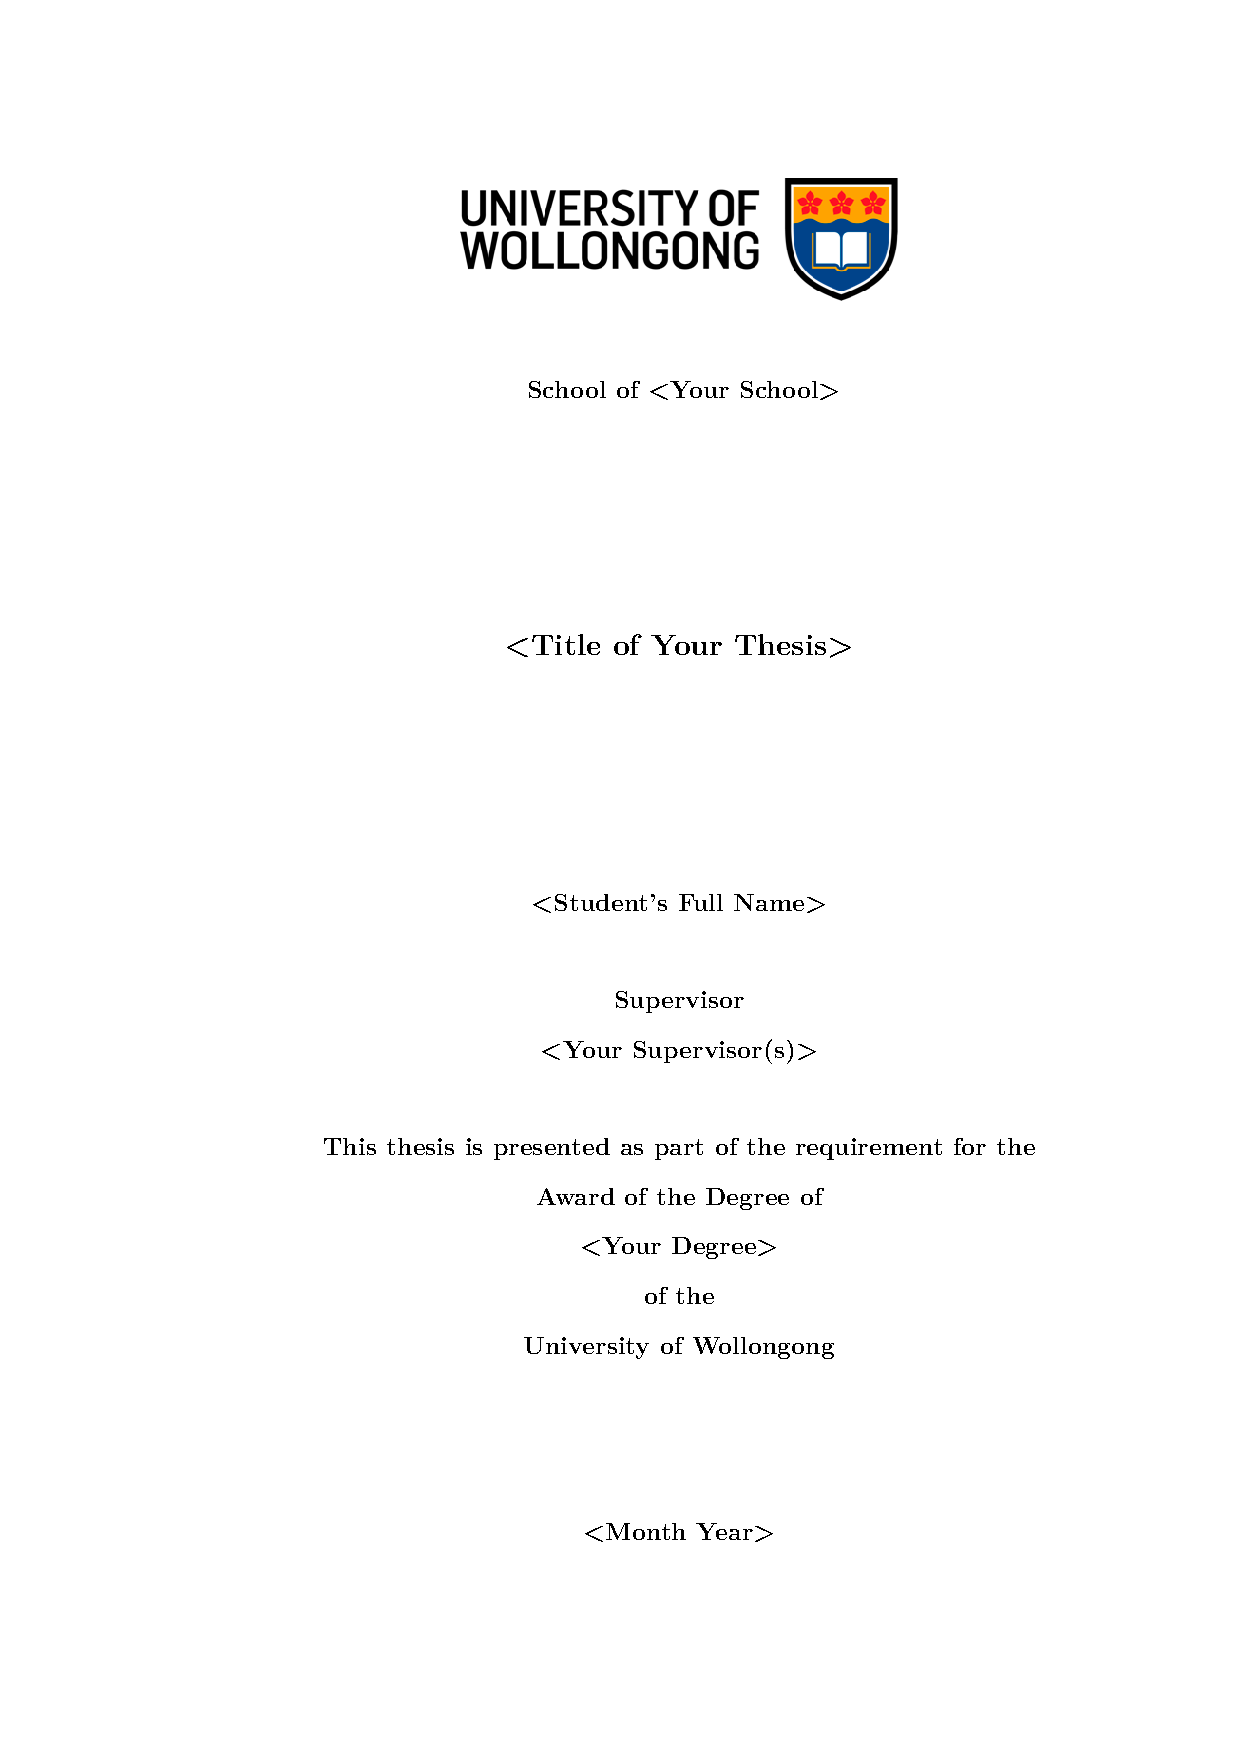
\includepdf{onesupervisor.pdf}
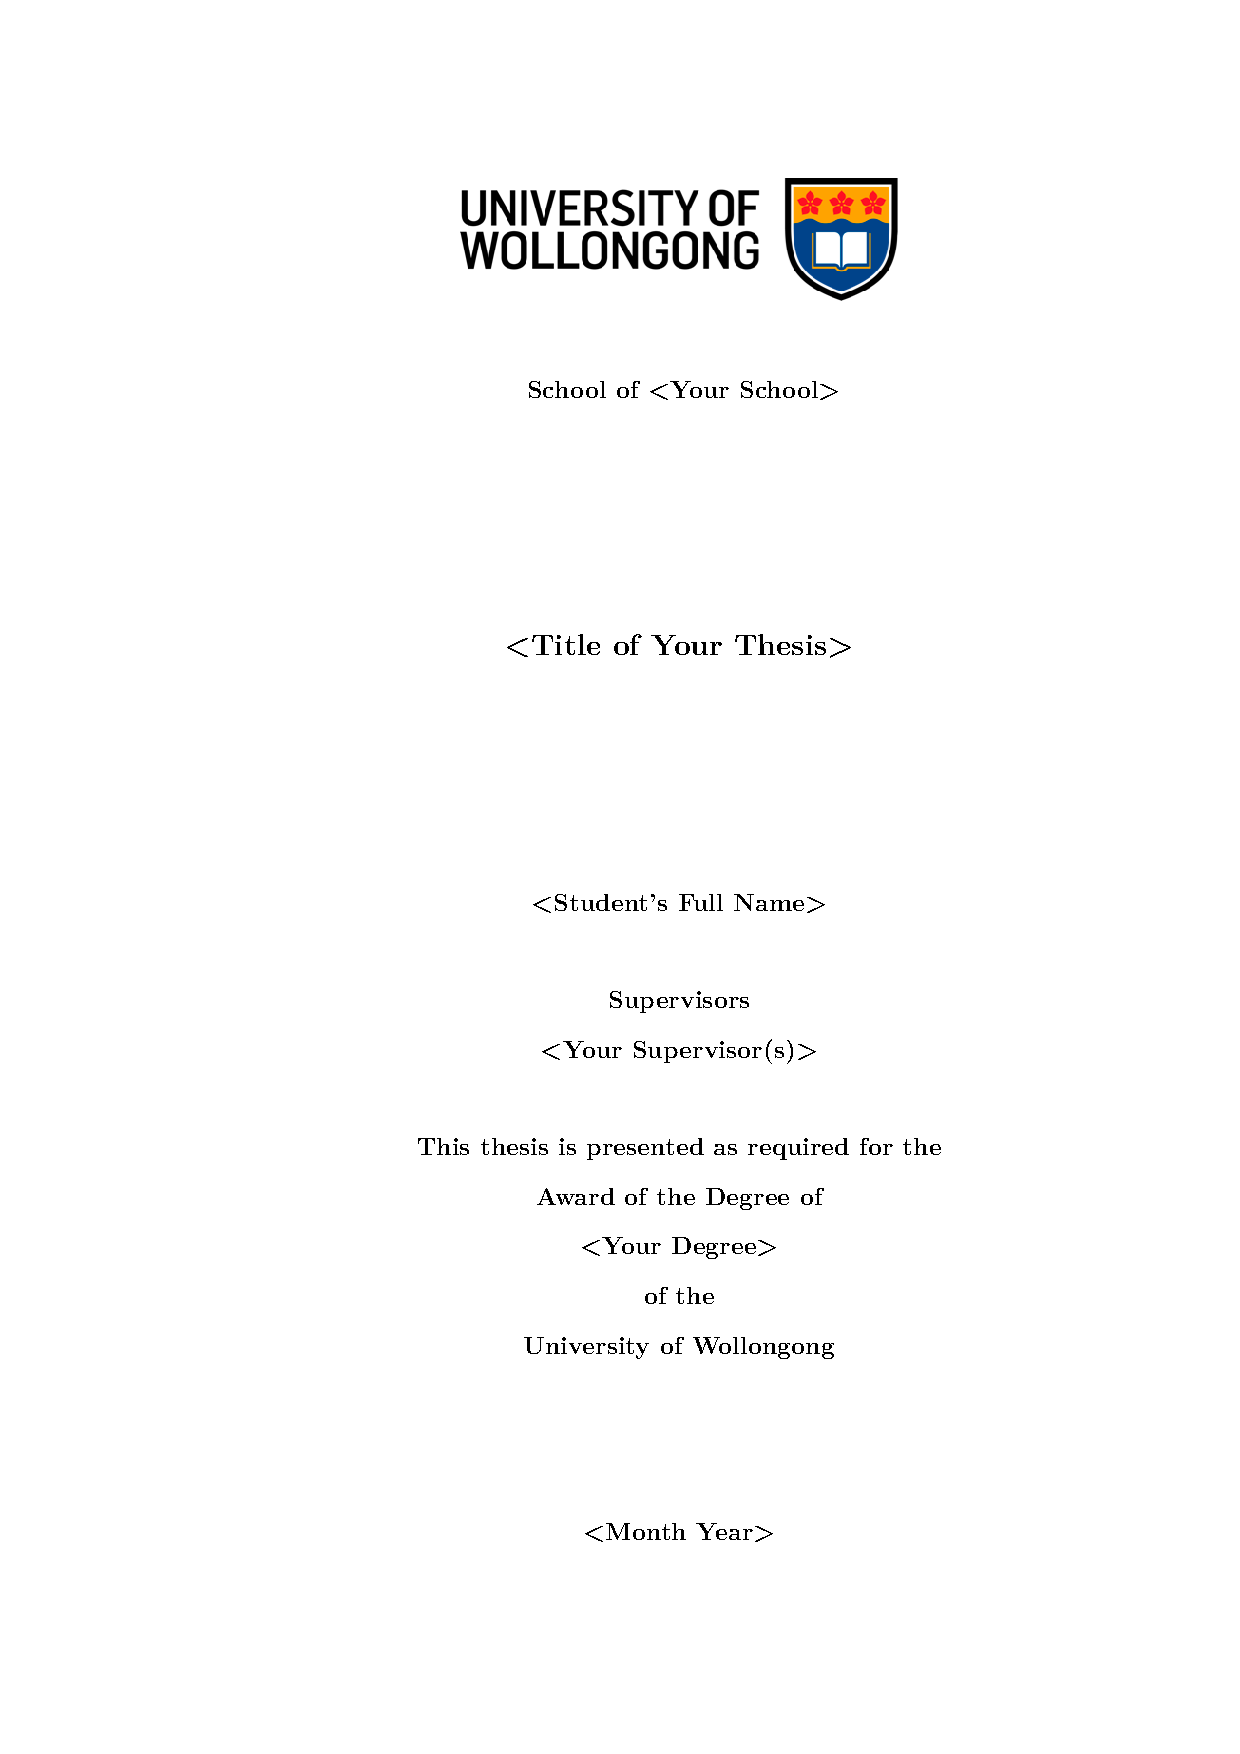
\includepdf{multiplesupervisors-phd.pdf}
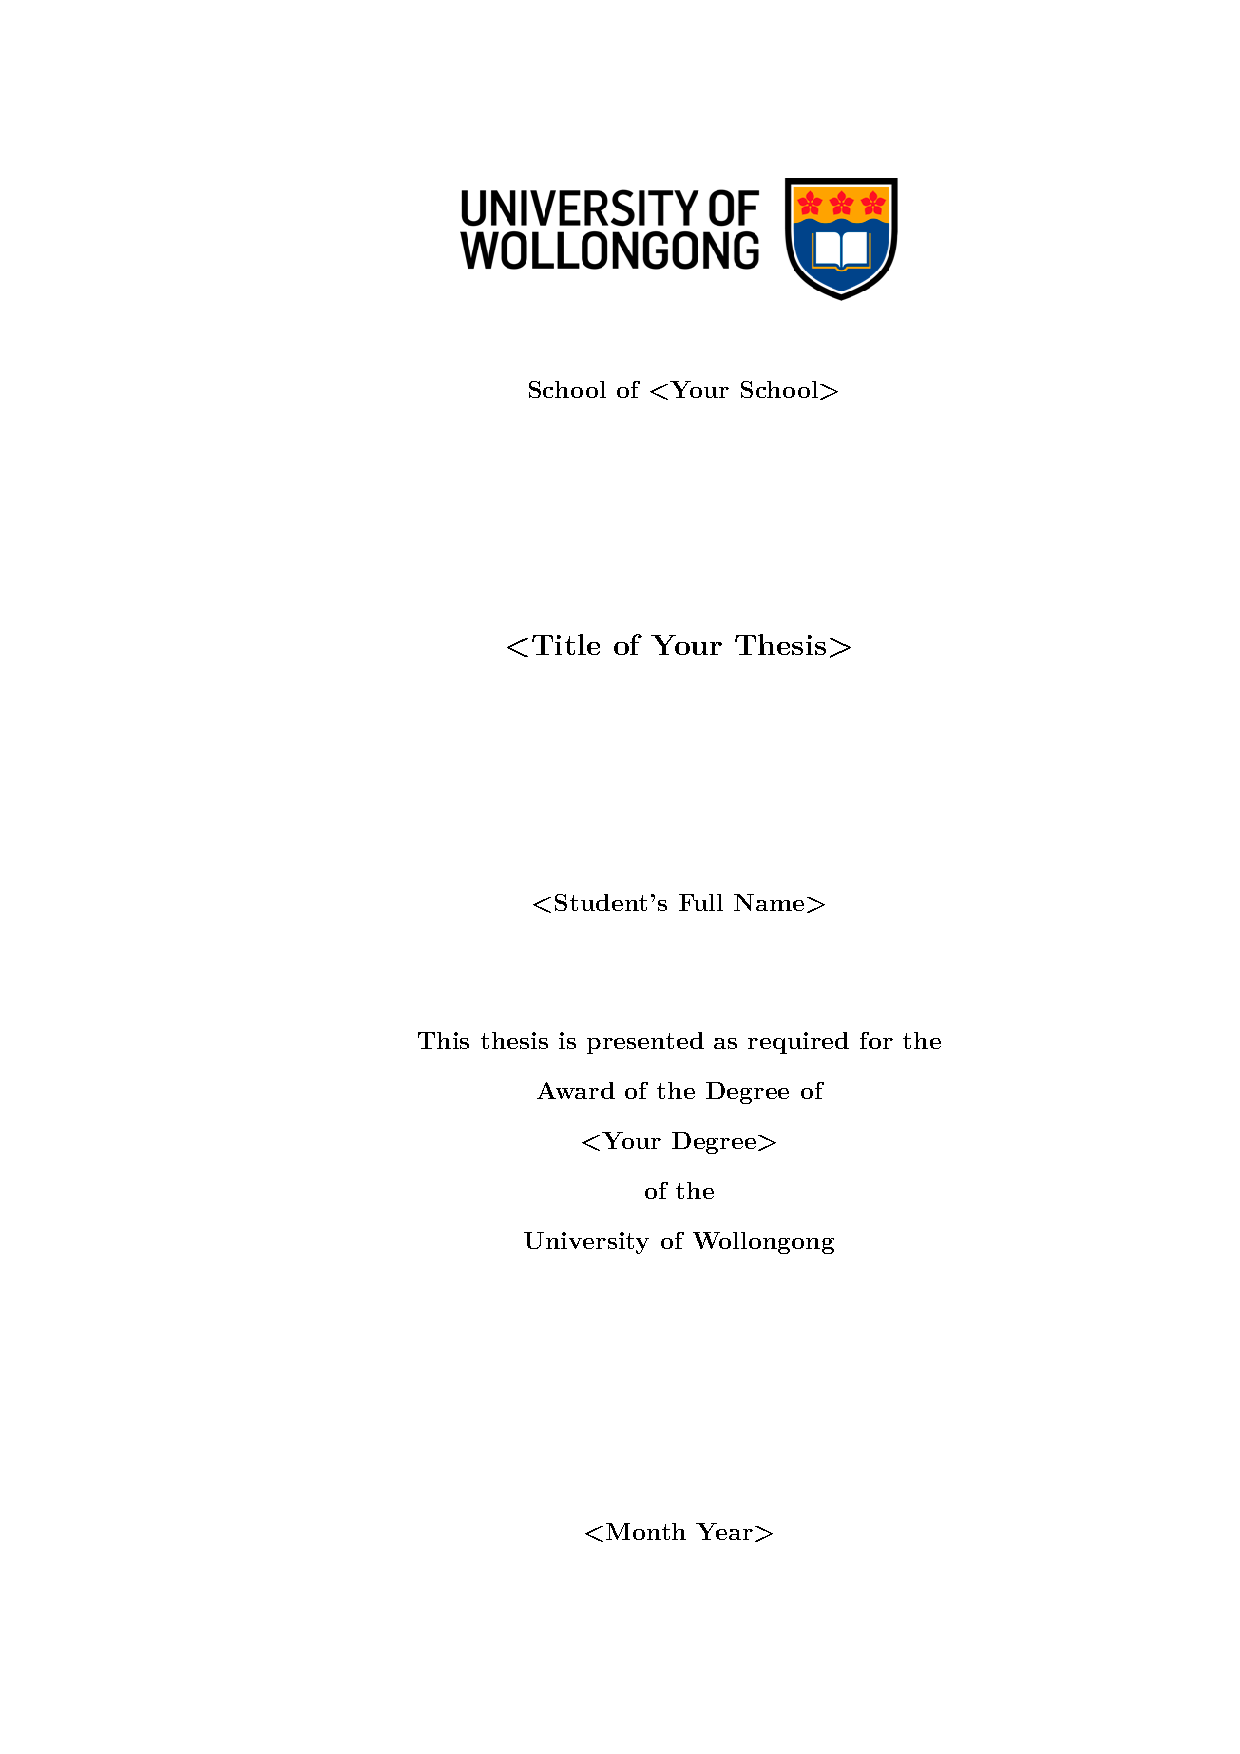
\includepdf{nosupervisor-phd.pdf}
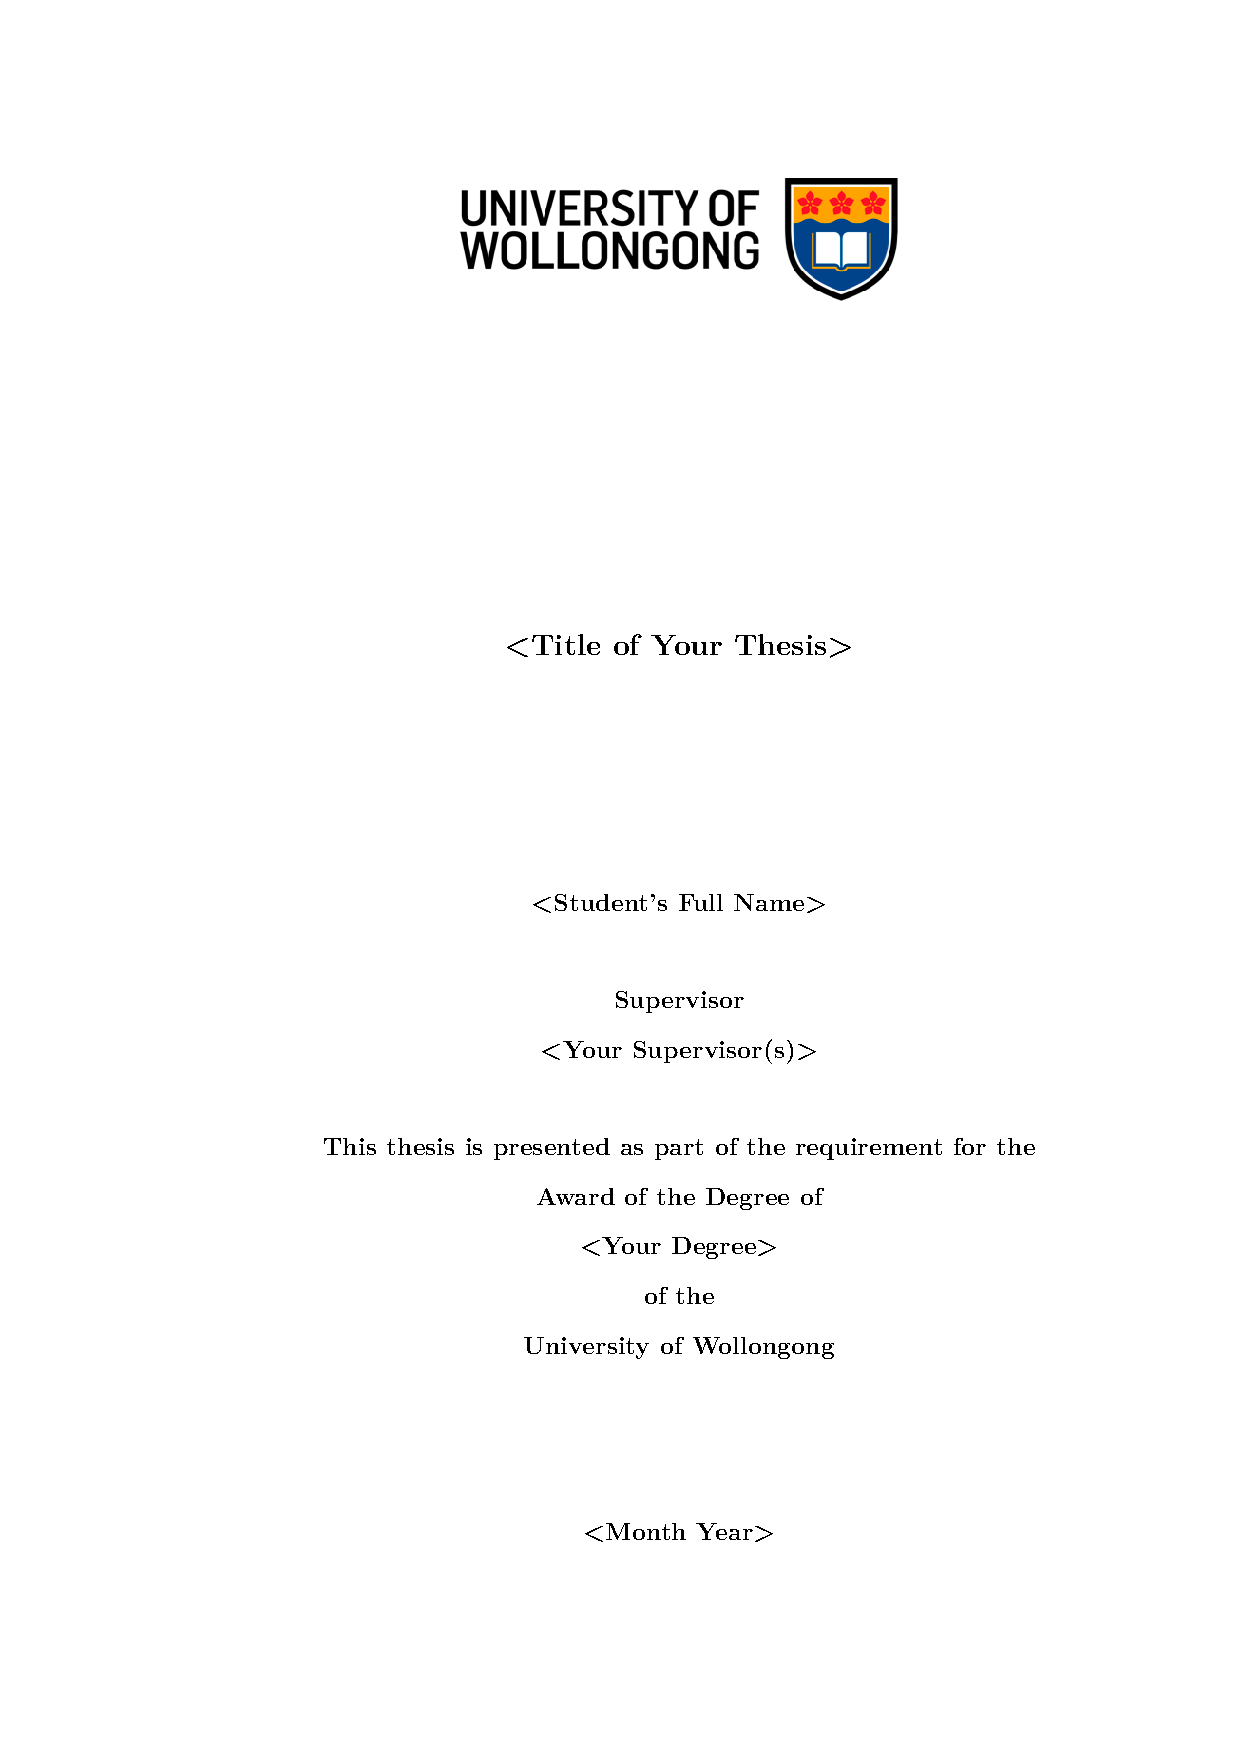
\includepdf{noschool.pdf}
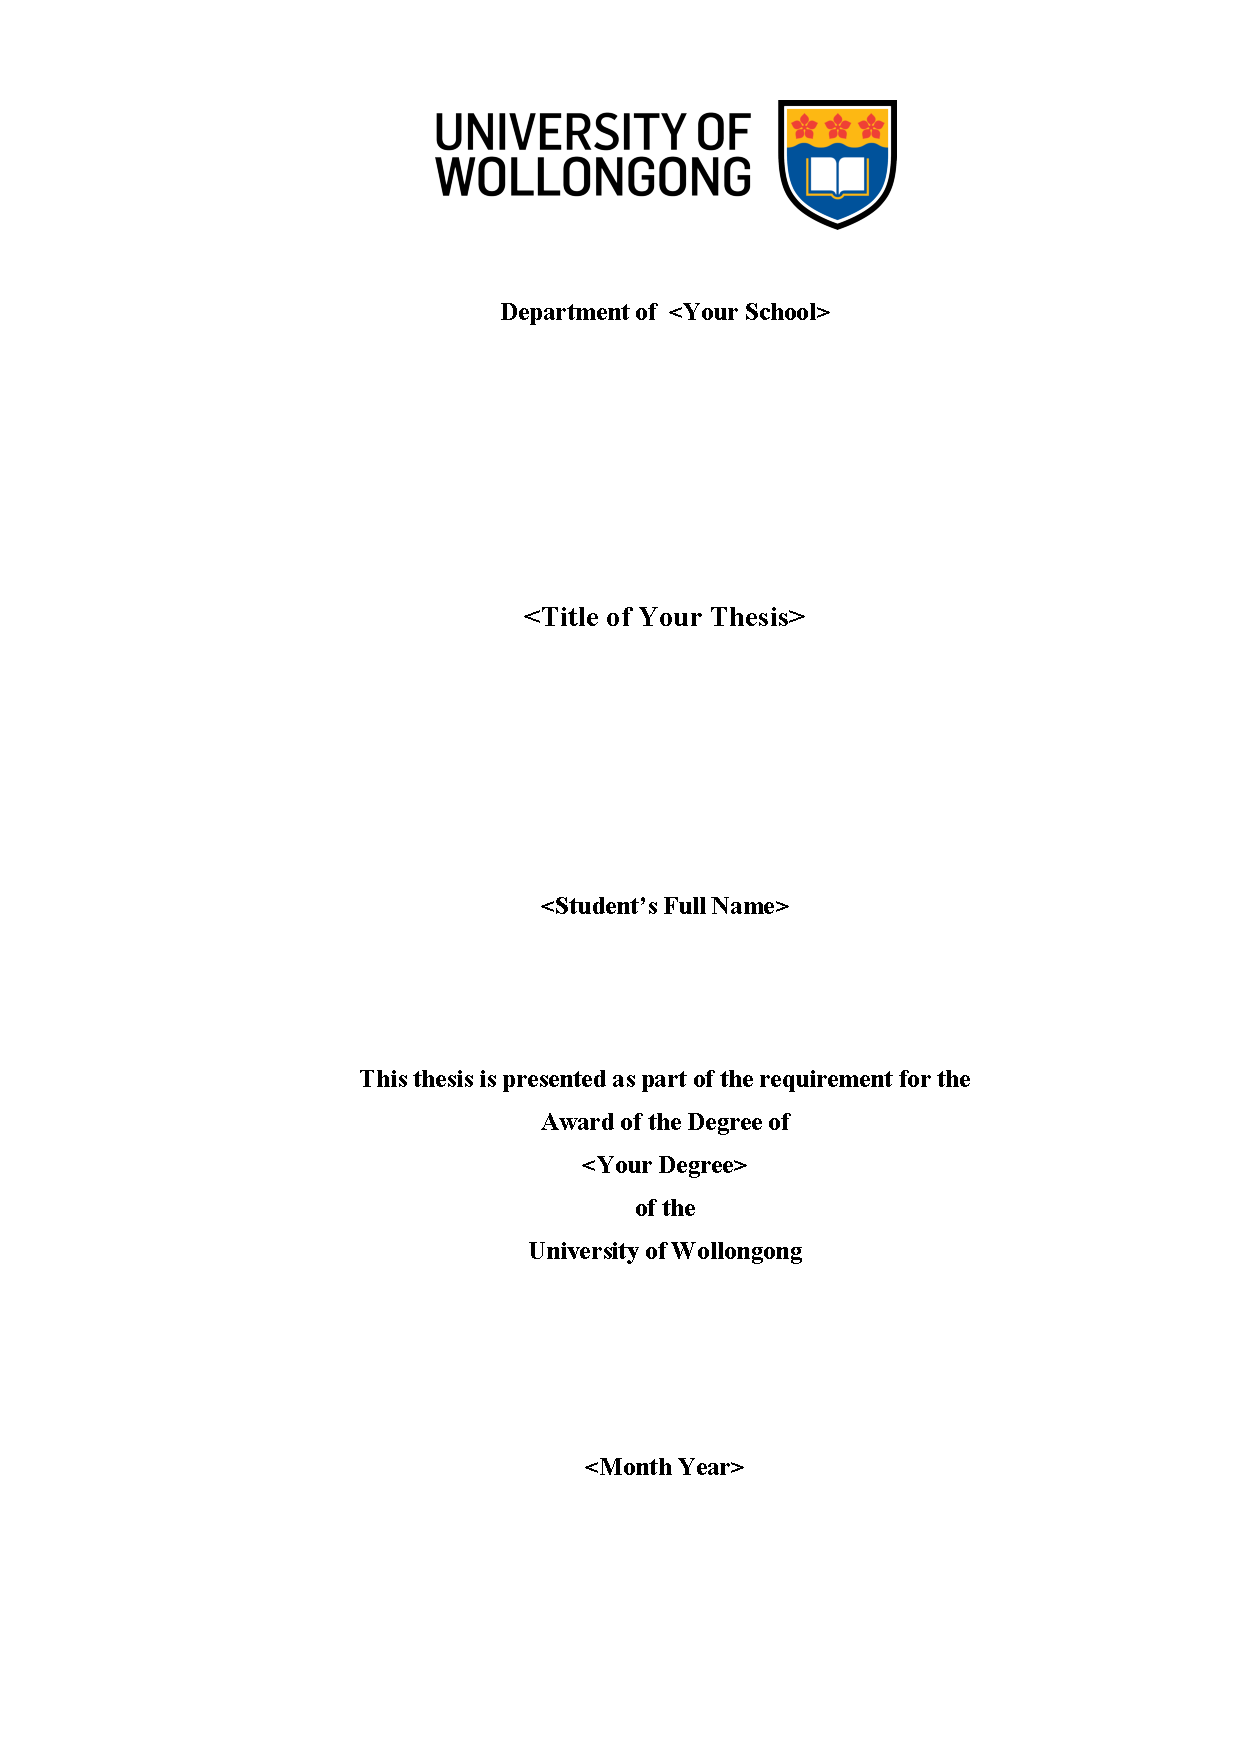
\includepdf{word.pdf}
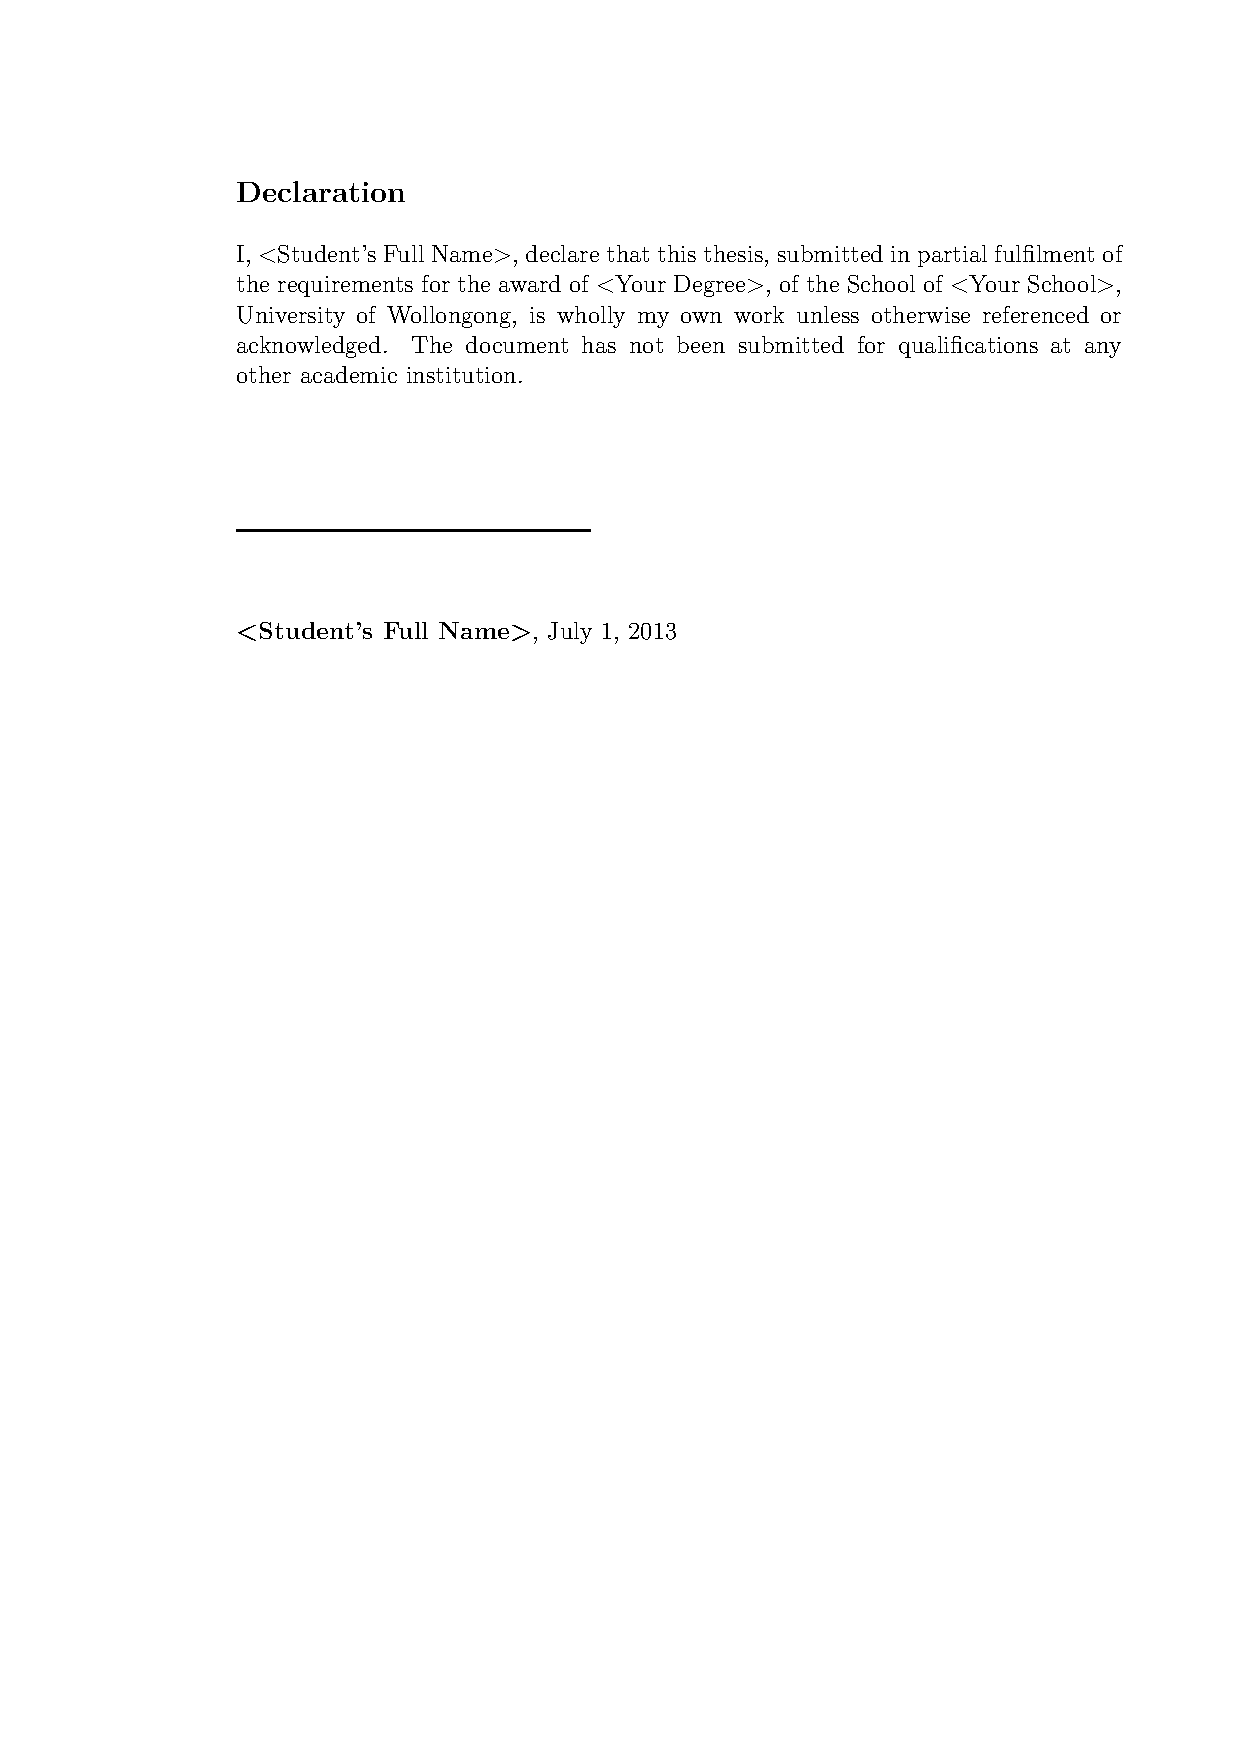
\includepdf{declaration.pdf}
\end{document}